\chapter{绪论}
\label{Intro}

\section{研究背景}

\subsection{社交媒体}
\label{ch1_social}
作为划时代的创新,互联网已经开始已深刻影响和改变着人类的生活、思维和行为方式。尤其现在,用户可以通过手机和各种穿戴式智能设备,随时随地保持与互联网不间断联系。根据中国互联网络信息中心的权威报告\footnote{\url{http://www.cnnic.net.cn/hlwfzyj/hlwxzbg/hlwtjbg/201407/P020140721507223212132.pdf}},截至2014年7月,我国网民规模达6.41亿,手机网民规模已超过5亿,互联网普及率已达到47.4\%\footnote{\url{http://www.cnnic.cn/hlwfzyj/hlwfzzx/qwfb/201408/t20140825\_47878.htm}}。
随着互联网技术的迅猛发展,网络进入Web2.0时代,出现了各种各样吸引广泛用户参与的社交媒体(Social media)平台。社交媒体逐渐开始将网络和人类社会生活融合在一起,已经开始成为工作、学习以及日常生活中必不可少的重要部分。
%图~\ref{fig1-1}展示了各种国内外的在线社交媒体平台。

%\begin{figure}[htp]
%\centering
%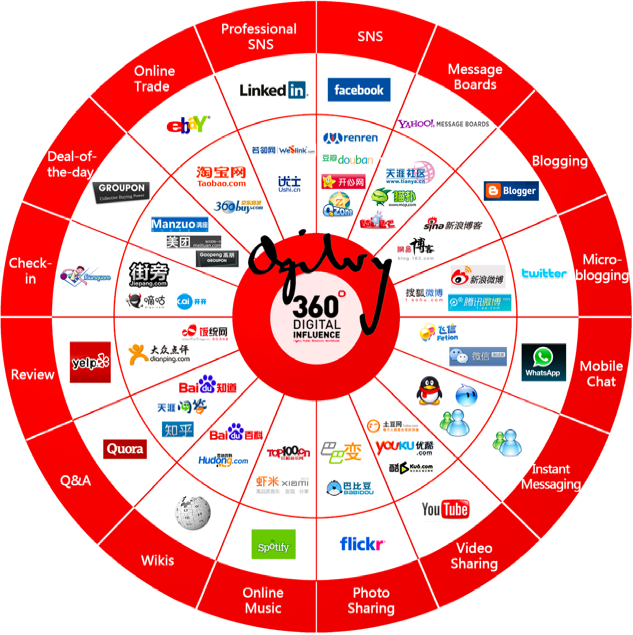
\includegraphics[height=340pt]{1-1.png}
%\caption{国内外社交媒体}
%\label{fig1-1}
%\end{figure}

Web2.0时代的互联网用户不再只是单纯的信息接收者,同时也成为网络内容的产生者,用户可以通过社交媒体进行交流而获取和产生信息。以中国为例,目前拥有12亿手机用户、5亿微博用户、5亿微信用户,每天信息发送量超过200亿条,交流无处不在,无时不有。表~\ref{tab1-1}是互联网网站信息统计公司Alexa\footnote{网站地址:\url{www.alexa.com},访问时间:2014年9月。}所做的网络访问量统计,从表中可以看出,流量前十的互联网网站中社交媒体就有七个。

\begin{table}[htp]
\centering
\caption{Alexa统计访问量前十名网站}
\label{tab1-1}
\begin{threeparttable}
 \begin{tabular}{|l|l|l|l|}
 \hline
 排名&网站&排名&网站\\
 \hline
 1& Google.com& 6&\textbf{ Wikipedia.org\tnote{1}}\\
 \hline
 2& \textbf{Facebook.com}& 7& \textbf{Amazon.com}\\
 \hline
 3& \textbf{Youtube.com}& 8& \textbf{Twitter.com}\\
 \hline
 4& Yahoo.com& 9& \textbf{qq.com}\\
 \hline
 5& Baidu.com& 10& \textbf{Taobao.com}\\
 \hline
\end{tabular}
\begin{tablenotes}
  \centering
  \footnotesize
\item[1]表中加黑的网站为社交媒体
\end{tablenotes}
\end{threeparttable}
\end{table}

那么究竟什么是社交媒体呢?社交媒体的典型代表维基百科是这样定义的\footnote{\url{http://en.wikipedia.org/wiki/Social media/}}:

\begin{definition}[Social Media]
Social media are media for social interaction, using highly accessible and scalable communication techniques. It is the use of web-based and mobile technologies to turn communication into interactive dialogue.
\end{definition}

从定义中可以看出,社交媒体是以网络技术和互联思维为基础的一项应用,用户因此可以非常方便进行内容创作、情感交流与信息分享。一般来讲,社交媒体可以分为如表~\ref{tab1-2}所示的几种类型。

\begin{table}[htp]
\centering
\caption{社交媒体的类型}
\label{tab1-2}
 \begin{tabular}{|l|l|}
 \hline
 类型& 代表性网站\\
 \hline
 维基(Wiki) & Wikipedia,Scholarpedia,百度百科\\
 \hline
 博客(Blogging) & Blogger,LiveJournal,WordPress,博客\\
 \hline
 新闻(Social News) & Digg, Mixx,Slashdot\\
 \hline
 微博(Micro Blogging) & Twitter,Google Buzz,新浪微博\\
 \hline
 评论(Opinion \& Reviews) & ePinions,Yelp,豆瓣\\
 \hline
 问答(Question Answering) & Yahoo! Answers,百度知道\\
 \hline
 媒体分享(Media Sharing) & Flickr,Youtube,优酷\\
 \hline
 书签(Social Bookmarking) & Delicious,CiteULike\\
 \hline
 社交网络(Social Networking) & Facebook,LinkedIn,MySpace,人人网\\
 \hline
\end{tabular}
\end{table}

如表中所示,社交媒体有多种不同类型,因此会产生多种不同形式的信息,主要包括文本、图像以及视频等。社交媒体上的信息由广大的社交媒体使用者产生,因此称为用户产生内容(User-Generated Content,UGC),这些信息依靠用户间建立的社交关系以及信息交互形成相互关联的庞大数据库。Kaplan和Haenlein\upcite{Kaplan2010}从信息产生和流动角度描述了社交媒体:首先是作为媒体(media),社交媒体最突出的特点是它区别于电视、广播和报纸等传统媒体(信息的流动是从少数内容生产者到广大的信息消费者),社交媒体中内容产生的权利扩展到了所有的用户,而且信息流动的方式变得不确定,用户可以在内容消费者和产生者之间不停地改变自己的角色;其次,之所以称这种新媒体是社会化的(social)的媒体,因为作为社交工具,社会化意味着信息内容不只是由个体用户产生,更多是与其他用户协作产生,信息的内容变得更加多样化,因此社交媒体不只是用来产生信息,更成为用户间信息交流、信息共享以及信息传播的便利工具。

虽然社交媒体的出现为用户沟通和交流提供了便利,但是随着用户数量不断增加,产生的内容不断达到新的量级,导致用户作为信息消费者遇到了一些新的挑战,用户从“信息海洋”中找到有用信息变得更加困难,这种现象称为信息超载(information overload)\footnote{信息超载描述了一种状态,就是当一个人在做选择时因为太多的信息而造成决策的困难。}。同时,由于社交媒体发布信息的快捷和方便,使得网络内容产生门槛降低,任何人都能够参与其中,因此社交媒体中的数据出现了不同于传统媒体数据的新特点。
一般来讲,社交媒体中的数据具有以下特点\upcite{eisenstein2013bad}:
\begin{itemize}
\item \textbf{数量巨大(Big)}:社交媒体中每个用户产生的数据可能不大,但是因为用户群体数量庞大,整体数据规模不可小觑,比如平均每天有超过300万条的微博(tweets)发布到Twitter\footnote{\url{http://www.twitter.com/}},每分钟有超过3000张照片上传到Flickr\footnote{\url{http://www.flickr.com/}},每年有超过160多万的博客(blogs)发表\upcite{Tang2014}。
\item \textbf{广泛链接(Linked)}:社交媒体的社会化特性使得用户产生的数据天生就是广泛链接的,最直观的表现就是用户产生内容由于用户之间的各种社交关系关联在一起,是一种新形式的大数据。这种关联的数据显然不是独立同分布的(Independent and Identically Distributed,IID),对于想要使用传统的数据挖掘和机器学习方法分析社交媒体的研究人员提出了新的挑战\upcite{jensen2002linkage,taskar2003label}。
\item \textbf{充满噪声(Noisy)}:社交媒体数据产生门槛的降低以及接入手段的增加,使得社交媒体的数据质量参差不齐,充满噪声\upcite{Agichtein2008}。不仅于此,社交媒体中的网络结构也充满噪声,主要是因为:一是网络中存在一些传播虚假和垃圾信息的用户\upcite{stringhini2010detecting};二是用户间建立关系的便捷性很容易使得用户将各种社交关系放在一起,并不区分好朋友和陌生人\upcite{xiang2010modeling}。
\item \textbf{非结构化(Unstructured)}:社交媒体中用户产生数据,特别是文本数据,是高度非结构化的。尤其是随着移动互联方式的普及,越来越多的用户使用移动设备更新Facebook\footnote{\url{http://www.facebook.com/}}的状态,发送微博,或者回复别人的帖子,这不但导致了文本内容短小,而且错误拼写频繁出现\upcite{rossion1999spatio},经常还有一些非自然语言的使用,比如表情符(:),:()和缩写(h r u(How are you))等\upcite{speriosu2011twitter}。
\item \textbf{不完整性(Incomplete)}:为了保护用户的隐私,社交媒体平台一般允许用户将一些个人数据进行隐藏不被他人看到,比如Facebook仅有很少部分用户(小于1\%)公开了他们的个人数据\upcite{mislove2010you},这些数据包括个人信息,状态更新,朋友列表,发布的视频和照片以及与他人的信息交流等有价值的内容,因此社交媒体的数据是极度不完整和稀疏的。
\end{itemize}

社交媒体的迅速普及与壮大,使得它在政治、经济以及教育等多方面发挥着越来越重要的作用。一些互联网公司以社交媒体大数据资源为支撑,以SaaS(Software as a service)形式为用户提供在线服务。典型的如谷歌和Facebook的自助式广告下单服务系统、Twitter基于实时搜索数据的产品满意度分析以及国内百度推出的大数据营销服务 “司南”等。同时,政府也是社交媒体数据的积极使用者,2013年曝光的棱镜门事件显示出美国国家安全部门在使用社交媒体数据强大实力,其应用范围之广、水平之高、规模之大都远远超过人们的想象。白宫2014年5月发布的《大数据:抓住机遇,守护价值》报告中重点提及了社交媒体大数据\footnote{\url{http://www.whitehouse.gov/sites/default/files/docs/big\_data\_privacy\_report\_may\_1\_2014.pdf}}。
社交媒体大行其道的今天,自然也会成为品牌营销的手段之一,比如今年世界杯的主要赞助商之一可口可乐就挑选了粉丝在Facebook和Twitter上分享的照片,尝试进行iBeacon在社交媒体营销中的运用。
目前常见的社交媒体的大数据应用有\footnote{来源:工业和信息化部电信研究院于2014年5月发布的《大数据白皮书》}:
一是基于用户个人信息、行为、位置、微博等数据而进行的个性化推荐、交叉推荐、品牌监测等营销类大数据应用,被互联网广告、电子商务、微博、视频、相亲等公司普遍采用。
第二,公共服务类大数据应用,即不以盈利为目的、侧重于为社会公众提供服务的大数据应用。典型案例如谷歌开发的流感、登革热等流行病预测应用能够比官方机构提前一周发现疫情爆发状况。国内也有搜索引擎公司提供诸如春运客流分析、失踪儿童搜寻的公益大数据服务。
三是积极借助外部数据,主要是互联网数据,来实现的一些相关应用。例如,金融机构通过收集互联网用户的微博数据、社交数据、历史交易数据来评估用户的信用等级;证券分析机构通过整合新闻、股票论坛、公司公告、行业研究报告、交易数据、行情数据、报单数据等,试图分析和挖掘各种事件和因素对股市和股票价格走向的影响;监管机构将社交数据、网络新闻数据、网页数据等与监管机构的数据库对接,通过比对结果进行风险提示,提醒监管机构及时采取行动;零售企业通过互联网用户数据分析商品销售趋势、用户偏好等等。

随着社交媒体的迅速发展与参与用户的数目不断增多,社交媒体中可使用的信息也越来越丰富,具有广泛的应用前景。但是社交媒体中信息的庞大规模使得手工分析其内容变得十分困难,因此本文从信息自动化处理的角度对社交媒体的信息,主要是文本信息进行挖掘与分析,发现有用的信息,为社交媒体的相关应用提供帮助。本文特别关注社交媒体中的观点信息,由于社交媒体与传统媒体存在显著的差异,其自身有不同的特点,本文将充分利用这些特点为解决观点分析与应用问题找到解决方案。


\subsection{观点分析}
%实际上文本信息有两种:事实信息与观点信息,事实信息是对事物的客观陈述。观点信息通常包含在博客、评论、回复或微博中,一般是由客户、读者或者公众用于表达表达自己的态度(attitudes),评价(appraisals),观点(perspective),情绪(sentiment)和情感(emotions)。用户不仅对产品(product)或服务(service)表达观点,也会对社会生活中各种话题(topic)或议题(issuses)表达自己的观点。
%观点挖掘或情感分析是自然语言处理(natural language processing)、机器学习(machine learning)以及文本挖掘(text mining)跨学科领域的研究,用于分析文本中对于产品、服务、话题或议题发表的观点,也称为情感分析或主观性分析(subjectivity analysis)\upcite{Liu2005}
%观点(opinion)一词起源于”opine“,通常”sentiment, view, feeling, belief, conviction, persuasion, notion, idea, and impression“为其同义词,词典中”opinion“被定义为信念,判断,个人的观点,态度,评价,思想,感觉和情感(belief , judgment , personal view, attitude, appraisal, thought , feeling, and emotion.)。观点的主要特点就是它是私人的感受,不是建立在证据和确定性基础上的。观点最终要有两个部分:目标(target)和情感(sentiment)\upcite{Liu2012}.
%实际生活中,别人的观点在决策过程中有时候是必不可少的信息。比如在商业领域,消费者在选择产品的时候常常需要知道其他人的对这些产品的评价,而商家为了市场营销也需要知道消费者的观点。在政治领域,投票者受到其他人关于候选人看法的影响而决定选择,同时大众的观点也会影响到政策制定者的政策决心。


信息分为两种,即客观信息和主观信息。语言学家Lyons\upcite{Lyons1977}将语言功能分为描述(Descriptive), 社交(Social)的和表达( Expressive)三种功能。其中描述功能主要表达客观事实信息(Factual information),而社交和表达功能往往表达的是个人的主观信息(Subjective information)。主观信息,在语言中主要表现为观点信息,是人们在语言中表达出的对于所谈论目标事物的态度、情感或者看法\upcite{Wiebe2004}。观点常常简化为对目标事物的认同或不认同(或者认为目标事物好或者坏,持积极(Positive)态度还是消极(Negative)态度)\upcite{Rachels1986}等简单表示形式。

以往为了获取用户观点,需要进行问卷调查,而社交媒体的出现,为用户提供了全新的内容共享平台,使大量连接到网络的用户能够在各种社交媒体发表和表达自己观点:例如用户可以在Amazon\footnote{\url{www.amazon.com}}, Yelp\footnote{\url{www.yelp.com}}, 以及TripAdvisor\footnote{\url{www.tripadvisor.com}}上发表各种商品和服务的评论,还可以在Twitter\footnote{\url{www.twitter.com}}和Facebook上对最新话题表达自己的观点。一般来讲,用户在社交媒体中表达观点的信息有三种类型:在评论、论坛、博客以及微博中针对某主题发表的个人体验(Experience)和想法(Opinion);关于新闻文章(Artitles)、议题(Isssues)、话题(Topics)发表的评论(Comments);在社交网站,比如Facebook上发表的个人状态更新(Status)。社交媒体因为拥有庞大的用户群以及用户产生的海量信息成为了观点信息的主要来源,利用社交媒体可以分析大众对各类话题所持的观点。
社交媒体中的观点信息无论是对个人还是机构都起到非常重要作用。比如Horrigan\upcite{Hoffman2008}发现社交媒体中信息的快速传播对于网络用户在某些话题上观点的形成具有深远影响,社交媒体用户表达的观点同样也是产品商家\upcite{Horrigan2008}以及政策制定者\upcite{Mullen2006}不得不考虑的重要因素,有证据显示这种观点的相互影响过程具有显著经济效应\upcite{Antweiler2004,Archak2007,Chevalier2006}。此外,大规模的用户意见整合形成的观点可以反映民众政治倾向\upcite{Tumasjan2010},甚至可以提高股票市场的预测效果\upcite{bollen2011twitter}。

社交媒体海量的用户产生内容不可能依靠人工地去发现和总结其中的观点信息,需要能够从文本中自动对观点信息进行挖掘和分析的计算方法。观点分析\footnote{本文中观点分析(Opinion analysis)综合了情感分析(Sentiment analysis),观点挖掘(Opinion mining)以及主观性分析(Subjectivity analysis)等任务,是对文本中的观点信息进行挖掘、分析以及总结的过程。}\upcite{Pang2008OMS}就是对文本中带有情感色彩的主观信息进行分析、处理、归纳和推理的过程,其目的是自动发现和区分针对目标的情感和观点,目标可以是命名实体、也可以是话题或事件。
尽管计算语言学和自然语言处理已经有很长的研究历史,但是直到2000年才开始进行观点挖掘和情感分析等观点分析任务的研究,此后观点分析一直自然语言处理非常活跃的研究领域。特别是由于社交媒体的出现,研究者首次拥有了大量带有观点信息的文本数据,也正是因为有了这些数据,规模性的观点分析研究才成为了可能。可以说观点分析与社会媒体是一同起步和成长的,是社交媒体中数据分析的核心研究。观点分析研究不仅对于自然语言理解(Natural language understanding)有着重要的影响,而且还对管理学,政治学,经济学和社会科学产生深远影响,因为这些领域都要受到人的观点信息的影响。

%
%
%观点分析(或观点挖掘)研究逐渐发展成为介于自然语言处理(Natural Language Processing)与自然语言理解(Natural language understanding)之间的一个独立领域,不像其他的自然语言处理任务(文摘或文本分类),观点挖掘主要处理与自然语言概念相关的语义信息和情感信息的推理而不需要对文本进行深度语法分析\upcite{cambria2014jumping}。

%如此巨大的信息量,主要是非结构化的(因为它是专为人类阅读消费产生的),因此不能直接使用机器处理的。文本的自动分析需要由机器对自然语言进行深入理解成,实际上本文距离这个目标还很远\upcite{6710245}。到目前为止,网上信息检索,汇总和处理都依据主要是依靠文本的文字表示方式。这些算法非常擅长于对文本进行检索,将其拆分,检查拼写和计算词语。但是,当涉及到解释的句子,提取有用的信息,他们的能力是非常有限的。这些基于词表示的算法的很大局限就是他们只能处理字面上的信息,而对于人类来讲,本文就不会收到这样的限制,因为本文看到的每一个字激活的语义相关概念,相关的情节和感官体验的级联,所有这些都使得本文可以以快速高效方式完成一些复杂任务(如词义消歧,文字蕴涵和语义角色标注)。计算模型试图通过模仿人类大脑处理自然语言的方式来弥补这样的认知差距,比如利用在未明确表示的文本语义特征。这些计算模型是有用既为科学目的(如探索语言交流的性质),以及用于实际用途(如能够有效地进行人机交流)。计算模型可以提供关于可再由心里语言学家(psycholinguist)进行探索的人类行为非常具体的预测。通过继续在这个过程中,本文可能最终会获得人类怎样进行语言处理深刻的理解。为了实现这样的梦想,需要具有前瞻性的思维心理语言学家,神经科学家,人类学家,哲学家,和计算机科学家的共同努力。
为了便于阐述,本文首先要针对观点分析研究中要用到的以下几个概念进行定义加以明确。
\begin{definition}[文档(Document)]
文档指的是自然语言中的文本片段,一般一篇文档中至少会讨论一个话题。
\end{definition}
\begin{definition}[话题(Topic)]
本文中的话题概念比较广泛,可以是命名实体,事件,或者文档中提及的抽象概念(政治、健康、体育等)。
\end{definition}
\begin{definition}[情感(Sentiment)]
情感指的是文档作者针对话题表达的态度(Attitude)、立场(Perspective)或情绪(Emotion)。
\end{definition}
\begin{definition}[情感极性(Polarity)]
情感极性指的是文档中对话题所持观点的情感倾向性,一般分为积极的(Positive)或消极的(Negative)情感。
\end{definition}
\begin{definition}[情感极性值(Polarity value)]
情感极性值指的是评价观点积极和消极程度的度量值,可以是一维的(打分值),二维的(积极值和消极值),也可以是多维的(喜怒哀乐等情感对应值)。
\end{definition}

对观点有不同的定义方法,例如Liu\upcite{Liu2012}将观点形式化定义为观点五元组$ (e_i,a_{ij},s_{ijkl},h_k,t_l)$,
其中$ e_i $是目标名称,$ a_{ij} $是目标的不同属性(或方面,Aspect),$ h_k$是持有观点的用户,$ t_l$表示时间,$ s_{jkl}$是观点的情感值。
Kim和Hovy\upcite{Kim2004}也对观点做了定义,认为观点由四个元素组成:即主题(Topic)、持有者(Ho1der)、陈述(Claim)以及情感(Sentiment)。
无论对观点如何定义,一般都认为观点分析就是发现和确定观点各个要素的过程。
总体来说,比较全面的观点分析可以认为是由三个主要步骤组成:
\begin{itemize}
\item \textbf{文本中观点信息识别}:需要识别文档中涉及的话题信息,将不同话题有关的文本片段按照话题对应关联起来,并且需要对文本片段进行主客观分类找到主观性文本,因为观点一般是从主观性文本中确定的。将主客观文本分离一般需要一些明显带有情感的词语作为特征,这些词语集合在一起形成了能对情感知识进行建模表示的情感词典。
\item \textbf{文本情感极性分类}:从文本中抽取有用的特征将文本分为不同的情感极性类别,一般是将文本分为积极或消极极性(或者中性,即客观文本),主要使用各种机器学习方法,或者使用基于规则的方法。
\item \textbf{观点的整合集成}:经过前面两步,得到了主观文本片段以及文本片段中的具体观点,观点整合集成是在更高的层次上观点分析过程,是将文本片段中分散的观点根据不同的维度合并,并按照不同的应用需求以合理的方式表示。比如将文本片段按照时间顺序串联起来形成观点随时间演化进行观点表示,或者将同一用户所有文本片段中的观点集成起来用以对用户的主观性进行建模。
\end{itemize}

观点分析有别于传统的话题分析,话题分析关心的是文本所阐述的客观话题,如文档是属于教育类还是娱乐类的;而观点分析主要是识别文档中表达的观点、喜好、立场和态度等主观信息,需要对文档进行语法、语义或者语用进行深入分析。在传统的话题分析中,主题词是最重要的特征,而在观点分析中,情感词是最重要的特征。观点分析涉及语言学领域的诸多问题,由于语言的复杂性和多样性,需要面临以下几个问题:

\begin{itemize}
\item \textbf{领域相关性}:某些情感词在不同的领域中具有不同的情感极性,比如 :``轻薄 '' 在通常意义下具有消极情感极性,如 ``举止轻薄'',而在电脑领域,``轻薄 ''却表示褒义,具有积极情感极性。
\item \textbf{语义歧义性}:比如某些词语具有多个词义,并且不同的词义常常呈现出不同的情感极性。比如``这款空调经济耐用''和 ``经济呈现快速发展'' 在这两句话中,``经济'' 具有不同的词性和情感极性,前者是形容词,具有积极情感极性,后者是名词,具有中性情感极性。
\item \textbf{上下文相关性}:语言中有许多词语本身是不具有情感极性的,但是在特定的上下文环境中,语言描述便具有了情感极性。比如:``小''、``高''、``快'' 等词语,在搭配组合``损失小''、``成绩高''、``进歩快''中,具有积极情感极性,但在搭配组合 ``心眼小''、 ``耗油高''、``耗电快'' 中,则具有消极情感极性。
\end{itemize}

%情感词典,是人们在表达观点时常用的一些词语,是主观性信息的最明显的证据(比如``好'')。无论对无监督还是监督方法,因此一部好的情感词典是从文本信息中发现主观信息的重要特征。近年来从网络数据中发现主观性信息变得越来越重要,能够获得大家对一些事物、人或事件的主观性态度比仅仅只有百科式描述更重要,比如对产品的问卷调查,政治选举的民调以及商业广告效果分析等。因此很多研究者开始注意到这种信息需求,并试图从网络数据中挖掘并分析主观性信息。然而大多数工作主要关注与于本中情感倾向的总体以及详细的分析,并且仅仅是对某些特定领域的文本数据,比如产品评论或博客,并不适用于其他类型数据。随着社交媒体的普及,用户可以更方便地发表与自己有关的信息,比如自己的生活和对周围食物的观点,这些越来越多的用户产生数据使得主观性信息的挖掘和分析变得更重要。受到这种趋势和研究需求的影响,TREC评测\footnote{\url{http://www.trec.state.tx.us/}}从2006年开始就有关于从网络信息中挖掘观点的评测,并且受到很多自然语言处理研究人员的关注。判断一片文档是否有主观性信息最简单直观的方式就是看看是否含有主观性词语,这种基于词语的判断方式的基本假设就是文档中含有主观性词语通常是表达作者的主观观点,比如在商品评论中出现``喜欢''通常表示作者喜欢这个商品。因此很多研究者研究了一些通过人工或自动方式产生带有主观情感倾向的词典。
%
%主要有两种类型的网络上的信息(即,事实和观点)。然而,目前的搜索引擎(如谷歌),都是为了表达同主题关键字的事实。Wiebie\upcite{Wiebe1994}将带有个人心理视角的文本称为主观性信息,相对于客观地叙述事件或描述虚构世界的文本。Dave等\upcite{Dave2003}提出了观点挖掘作为从网络数据中发现主观性信息的研究。观点是所有人类活动的中心因为观点是本文行为的关键影响因素,本文对现实世界的感知和看法是建立在他人是怎么看这个世界的基础上的,当本文做决策之前通常会寻求其他人的观点。随着社交媒体的出现并流行(评论,论坛,博客,微博,评论,以及在社交网络中的帖子等),带有主观性信息的数据爆炸式增长,因此本文对观点信息的获取不再需要靠传统的问卷调查等手段。然而发现并综合各种社交媒体中观点信息并不是意见容易的事,因为数据量非常大之外,人工阅读并发现主观性信息是不可能的,因此需要自动观点挖掘技术。近年来,在社会化媒体带有主观性信息的贴子在本文的现实生活中帮助重塑了企业,并左右公众的情绪和情感,这对本文的社会和政治制度深刻影响。这样的帖子对于鼓动群体运动引起政局变化具有很大作用,比如2011年发生在一些阿拉伯国家的阿拉伯之春运动。因此收集和研究在网络上的意见成为一种必然。情感分析应用已经普及到几乎所有可能的领域,从消费产品,服务,医疗保健和金融服务等社会活动和政治选举。除了现实生活中的应用,很多应用为导向的研究论文也已发表。例如,情感信息可以预测产品的销售量\upcite{Liu2007},电影的票房\upcite{Oghina2012,Joshi2010,Sadikov2009,Asur2010},股市走向\upcite{Zhang2011,bollen2011twitter},政治选举的结果\upcite{Tumasjan2010,Chen2012,Metaxas2011,Gayo-Avello2011,Armstrong2011}等等。
%
%由于具有许多挑战性的研究问题和广泛的实际应用价值,观点挖掘和情感分析在过去的十年一直是非常活跃的研究领域。所有情感分析研究围绕一系列的任务,包括极性分类\upcite{Pang2004},观点抽取\upcite{Ding2009}以及观点源设定\upcite{Zhao2010}。
%
%大多数方法严重依赖于标注语料训练情感分类器,因此情感标注语料可以说对情感分析是非常珍贵的资源。本章最重要的一个目标就是减轻费力的标注过程,发展一种无监督的情感分析方法。
%
%在文本情感分析中,中文与英文的分析方法有所不同,中文首先要解决文本切词的问题,其次在特征提取方 法和情感词典构建等方面都存在一定差异。目前国内针对中文情感分类的研究相对较少,有采用类似英文情感分类方法的研究,朱嫣岚等人利用知网计算待定词与基准词间的相似度来判断其倾向性\upcite{朱嫣岚2006}。
%然而过去的情感分析研究主要是针对英文社交媒体(比如review以及Twitter),很少有工作致力于中文社交媒体的研究,就本文所知,在对中文微博的研究中,主要是开始进行一些基本的介绍和预测\upcite{Guo2011,Yu2011},近些年开始进行特点分析\upcite{Tian2012}以及用户微博行为分析\upcite{Gao2012,zhang2008review}。本文中,本文特别关注于中文的情感分析尤其是微博和产品的评论,进行了一下方面的研究(1)通过分析中英文情感词典的不同特点,根据情感知识相通的前提,使用语义知识词典根据对应语义关系将英文情感词典的情感知识转移到中文词语形成新的中文情感词典,减少了人工区分和标注;(2)研究英文情感词语的扩展方法在中文环境下的性能,并根据中文特点提出相应的语法特征以及统计特征,通过混合方式在中文社交媒体语料中扩展和构建情感词典;(3)基于使用机器学习方法进行情感分类框架,依据中文中情感表达的特色,对情感分类特征空间进行改进,更新分类模型,提出了一种无监督的中文微博情感分类方法。
%
%与事实信息为基础的分本分类相比,观点信息的分类通常类别会少一些,可能只包含正面负面情感极性(sentiment polarity)或者序号类别(ordinal categories),因此观点信息的抽取一般是关注于观点表达方式抽取(比如情感类型以及强度),比事实信息抽取(话题、事件、实体等)相对来讲看起来好像简单,实际上并非如此。事实信息因为与话题相关的关键词的不同而在不同话题的文本中差别很大,因而容易区分,可观点信息并非如此,因为情感的表达是以一种细致的方式表达,因而单靠只言片语很难确定,需要以来与具体的上下文语境,同一个表达方式在不同领域可能表达了不同的情感类型。这些都是观点信息分析的挑战和吸引之处。
%
%总体来讲,情感分类研究可以分为基于词典和基于学习的。简单来说,基于词典的方法是使用人工或者自动编辑的词表(比如“喜欢”等),并认为这些词语的出现是观点的标志;而对于学习方法来说,主要是依靠词语共现来使用已有分类的数据实例来训练产生分类器进行自动分类。

\section{研究问题}
\label{point}
随着以Twitter,Facebook、新浪微博为代表的社交媒体迅速发展,人们越来越愿意在线分享自己的看法、观点以及体验,他们可以选择博客写作、微博发帖、社交网络状态更新、发表产品评论、或者在论坛中参与讨论等方式发表对于关注话题的看法和观点,因此网络充满了各种意见,现在的网络可以说是一个“观点网络”,网络已经成为获取观点信息的主要来源。但是站在网络使用者的角度,一方面可以很容易获得大量的带有观点的信息,这些信息远远超出了个人的信息消费能力,因此用户面临着“信息超载(Information overload)”问题;另外一方面,观点的主体是人,而网络中的信息尤其是社交媒体中的信息多是以“碎片化”的形式存在,每个人观点分散在信息碎片海洋中,因此满足用户真正的信息需求(能针对目标主题快速准确地从网络中找到需要的观点)变得更加困难,因此用户又面临“信息不足(Information shortage)”问题。传统的信息检索技术,比如搜索引擎,很难解决这样矛盾的信息供求关系。当然目前已经有观点检索系统\upcite{he2008effective,macdonald2007overview,ounis2011overview},可以解决如“检索评价某产品的文档,并总结其中的观点”这样的问题,但是还不能满足“查找大家对某产品的观点或某个朋友对该产品的观点”这样的信息需求。因为这样的问题需要就网络中,尤其是社交媒体中每个用户的观点进行挖掘、分析并整合集成。网络中的信息,一个事实信息可以代表所有的事实信息(One fact stands for all facts),但是一个观点不能代表所有的观点(One opinion can not represent all opinions)。
从信息产生者的角度来说,用户一条信息中的观点可能只是他就话题的某个方面表达出的观点,就话题整体的观点需要将所有分散在“信息碎片”中的观点进行集成,并以一种合理的形式表示出来,才能代表用户对于话题的完整观点。
因此本文首先从下面一个科学问题出发,来研究观点分析:

\textbf{科学问题1:怎么样才能准确从社交媒体碎片化文本信息中分析得到用户层面的观点信息?}

这个问题需要从挖掘用户产生的信息碎片中的观点出发,是一个观点信息确定、分类以及整合的过程,需要解决文本情感知识表示,情感极性分类以及观点信息集成等问题。

从另外一个角度来看,人是具有主观能动性的,人的行为会受到自己观点和看法等主观性的影响。用户在使用社交媒体时会有多种交互行为,比如信息传播行为,人们通过转发分享新闻与观点,加速信息的流动、扩大信息传播的范围。用户的信息传播行为同样会受到自己的主观性的影响,通过观点的分析与与集成可以对用户的主观性进行建模分析,而用户的主观性模型无疑会对分析用户的一些在线的信息交互行为分析有帮助。因此本文从以下两个科学问题出发来研究用户的主观性建模,并分析其对用户在线交互行为的影响:

\textbf{科学问题2:用户的主观性如何表示和建模?}

\textbf{科学问题3:怎么样使用主观模型分析用户的在线交互行为?}

用户在社交媒体中的产生的内容会涉及到多种话题,而且会对话题的不同方面发表观点,因此回答第一个问题需要研究用户产生信息中多样性话题的确定及表示问题,还有用户在不同话题上多方面观点的集成及表示问题。
在使用社交媒体过程中,用户作为带有自己主观判断的主体,会在不同情况下产生不同的交互行为,因此回答第二个问题需要首先确定用户在线交互行为产生的具体原因,然后研究怎么样从主观动机角度对这些原因进行度量分析。

\section{相关研究}
本节主要介绍观点分析与用户传播行为分析相关的一些现有工作,其中观点分析包括观点挖掘和观点集成两个部分相关工作。
本文的相关工作分析主要从整体相关工作和局部相关工作进行阐述,本章的相关研究主要介绍的是整体的相关工作,因为这些研究成果可以为本文所研究的具体任务提供思想借鉴和技术支持。以后各个章节中的相关工作则会具体地分析已有的类似工作以及研究成果。
特别需要强调的是,无论是观点分析还是行为分析,对社交媒体中文本的处理都是其中一个重要的环节。社交媒体数据的一些特性已经在第~\ref{ch1_social}节有所介绍,这些特性造成自然语言处理技术在社交媒体上的应用存在着新的挑战,使用自然语言处理技术对社交媒体文本进行处理,主要工作包括文本规范化(Normalization)\upcite{eisenstein2013bad,toutanova2003feature,gimpel2010part,owoputi2013improved},领域适应化(Domain adaptation)\upcite{finkel2005incorporating,ritter2011named,foster2011news,
han2011lexical,han2012automatically,han2013lexical,liu2012joint,liu2012broad,Hassan2013,gimpel2010part,owoputi2013improved,finin2010annotating,
ritter2011named,liu2011recognizing},预处理(preprocessing)\upcite{li2012twiner,liu2012joint,liu2013named}以及进行一些结构化处理(词性、句法、标注等)\upcite{liu2012two,sharifi2010summarizing,chakrabarti2011event,
takamura2011summarizing,weng2011imass,harabagiu2011relevance,Ren:2013:PTT:2484028.2484052,shen2013participant,judd2013better,chang2013towards,
finin2010annotating,ritter2011named}。本文在进行观点分析研究时,需要借鉴已有工作对社交媒体的非结构化噪声文本进行预处理,但是这些预处理方法不属于本文研究内容,因此不作详细介绍。

\subsection{观点挖掘}
\label{ch_mining}
观点挖掘研究主要是识别文档中针对某一话题表达出的观点并判断观点的积极或消极极性\upcite{Liu2012}。观点挖掘通过对文档深入分析得到文档中表达的观点信息,是观点集成等后续分析任务的基础,观点挖掘的准确性影响着后续分析任务。一般来说,观点挖掘包含观点识别(Identify)和极性分类(Classify)两个步骤。观点识别是从文档中识别出话题以及与话题相关的观点文本片段。识别带有观点的文本片段(一般是文档中的句子)也称为主客观分类(Subjectivity analysis),是将文档中的带有观点信息的句子与描述客观事实的句子区分开,有研究表明将文档中的主客观文本分类后,使用主观部分有助于提高观点挖掘的准确性\upcite{Schler2005}。目前主客观分类主要采用各种机器学习方法进行分类\upcite{Wiebe2001,Wiebe2005,Dave2003,Pang2004,Riloff2005,Wilson2009}。极性分类是将文档就话题表达出的情感极性进行分类,一般是分为积极与消极极性,也可以是多种类别(当类别为积极、消极以及中性时,与主客观分类一致)。
观点挖掘研究方法可以分为基于词典方法、基于特征共现统计方法以及基于机器学习方法等三类。

\subsubsection{基于词典的观点挖掘}
基于词典的观点挖掘依赖于预先构建好的情感词典,词典里的词语都标注了相应的情感极性(值)。常用的英文情感词典有General Inquirer\footnote{\url{http://www.wjh.harvard.edu/~inquirer/}},DAL(Dictionary of Affect of Language)\footnote{\url{http://www.hdcus.com/}},WordNet-Affect\footnote{\url{http://wndomains.fbk.eu/wnaffect.html}}以及SentiWordNet\upcite{Baccianella2010}。
基于情感词典的方法用词典确定文档中的带有情感极性的词语,以判断文档是否主观文本。一些研究使用情感词典词语的情感极性值来进行文本情感极性分类\upcite{Angel,Tsytsarau2010,Missen2009}。一个句子或文档的情感极性值可以通过将每个词语的极性值取平均来确定,常用的计算方法可以使用公式~\ref{eq1-5}来表示:
\begin{equation}
\label{eq1-5}
S(D)=\dfrac{\sum_{w \in D}S_w \ast weight(w) \ast modifier(w)}{\sum weight(w)}
\end{equation}
其中$ S_w $是文档中的词语在情感词典中的极性值,$ weight(w) $是权重函数,可以根据词语相对于话题词的位置进行权重调整,$ modifier(w) $是专门处理否定、增强或其他改变词语情感值的一些修饰操作函数。
典型工作如Zhu等\upcite{Zhu2009}首先将文档或句子中词语的极性值累加在一起,然后使用简单的基于规则方法计算整个文档或句子的极性值。一些比较成熟的情感分析工具,比如Sentiment Analyzer\upcite{Yi2003},或Linguistic Approach\upcite{Thet2009}针对话题挖掘一些领域相关特征、观点句的模式或词性标签等作为规则加入到文档极性值的计算中,可以得到更精确的极性值,但是会增加计算复杂性。

\subsubsection{基于特征共现统计的观点挖掘}
这种方法是基于语料中表达相似观点的词语经常会在一起出现这一假设基础上的。如果两个词语频繁在同一上下文中同时出现,它们就很有可能有相同的极性。因此一个词语的极性值可以根据它与一些极性恒定的词语(比如“good”)共现的频率来确定。Turney\upcite{Turney2002,Turney2003}提出使用点对点互信息(Point-wise mutual information (PMI))\upcite{Church1990}作为统计依据来计算词语的共现:
\begin{equation}
PMI(x,y)=\log_2\dfrac{F(x,y)}{F(x)F(y)}
\end{equation}
其中$ F(x,y) $表示两个词语的共现频率,$ F(x) $表示词语$ x $的出现频率。词语$ x $的极性值可以通过计算该词语与两个相反极性基准词语的互信息差值来确定:
\begin{equation}
PMI\_IR(x)=\sum_{p \in pWords}PMI(x,p)-\sum_{n \in nWords}PMI(x,n)
\end{equation}
其中$ pWords $表示积极极性的基准词集合,$ nWords $表示消极极性基准词集合。为了统计词语出现频率,Turney使用AltaVista搜索引擎检索词语返回的条目数作为词语出现频率。Chaovalit和Zhou\upcite{Chaovalit2005}扩展了Turney方法,通过谷歌搜索引擎确定词语共现频率,提高了准确性。Read和Carroll\upcite{Read2009}使用语义空间相似性和分布相似性作为替代方法进一步扩展了Turney方法。对这种方法全面的研究是Taboada等\upcite{Taboada2006},他们指出了使用搜索引擎确定共现频率可能会存在的一些问题。Ben等\upcite{he2008effective}提出使用统计方法构建情感词典与信息检索相结合的方法获取主观性博客文档。

\subsubsection{基于机器学习观点挖掘}
在观点挖掘研究早期,机器学习方法和标注数据集的使用加速了研究的进展,目前观点挖掘最常使用的仍然是机器学习方法。机器学习方法是对分类问题的比较成熟的解决方案,一般经过训练和预测两个过程,可以进行如下形式化表示:假设训练数据集是经过极性标注的文档集$D$,每个文档都可以用特征(词语,二元组等等)向量表示,文档都被标注了情感极性(在极性空间$S$中的一个值),机器学习的训练过程可以形式化为,给定训练数据集:$ \{(d,s)|d \in D,s \in S\} $,找到映射:
\begin{equation}
g:D \rightarrow S,\quad g(d)=\arg max_S f(d,s)
\end{equation}
极性分类也就是找到映射$ g $,将文档根据打分函数$ f $映射到情感极性空间$ S $,函数$ f $以文档向量和标注的极性作为输入,对未标注的文档给出极性预测的概率值(使用条件概率或联合概率),训练的过程就是对打分函数$ f $的估计过程。一般机器学习方法有以下几个步骤:
(1)首先获取训练数据集,数据集可以是带标注的(有监督),也可以是无标注的(无监督);
(2)在文档集中抽取有用特征,将文档使用特征向量表示;
(3)通过分析相关特征共现规律,训练分类器区分文档集极性标注;
(4)最后使用训练得到的分类器对新文档极性预测给出概率值。

Pang和Lee\upcite{Pang2002}最先将机器学习方法引入了观点挖掘领域,作者提出了使用三种有监督的分类器(Naive Bayes (NB),Maximum Entropy (ME)和Support Vector Machines (SVM))进行电影评论的情感极性分类,实验结果显示三种分类器性能都超过随机选择的基准分类器,平均准确率达到80\%,其中SVM表现出最好的性能。Dave等\upcite{Dave2003}扩展了Pang的工作,强调使用特征选择对情感分类特征进行过滤,可以将准确率提高到87\%。Pang和Lee\upcite{Pang2004}使用主客观分类对文档进行预处理,过滤掉其中的描述客观信息的句子,发现可以提高极性分类的准确性。后续的一些工作主要集中于研究如何发现有用的分类特征\upcite{Melville2009,Vegnaduzzo2004,Devitt2007,Osherenko2007},训练数据的构建\upcite{Goldberg2006,Taeckstroem2011}以及机器学习方法的选择\upcite{Mcdonald2007}。

\subsection{观点集成}
\label{ch_integrate}
通过观点挖掘得到的是单个文档中的观点信息,很多实际应用关注的是更高层次的观点,而不仅是单个文档的观点,因此需要对文档观点分析结果进行整合集成。这种整合集成可以按照不同的维度进行,比如为了了解一群人的观点分布,需要将每个人发表的所有文档中的观点进行集成。最需要观点集成的研究领域是产品评论,需要从大量用户发表的评论中抽取出产品的特征,并计算不同用户针对相同特征的观点或打分的平均值,以此进行观点集成形成对产品总体的评价。以图~\ref{fig1-2}所示产品评论的观点集成为例\upcite{Tsytsarau2012},观点集成一般包括信息收集,观点识别,观点分类以及推理集成三个步骤\upcite{Tang2009,Liu2005,Ng2006}。
\begin{figure}[htp]
\centering
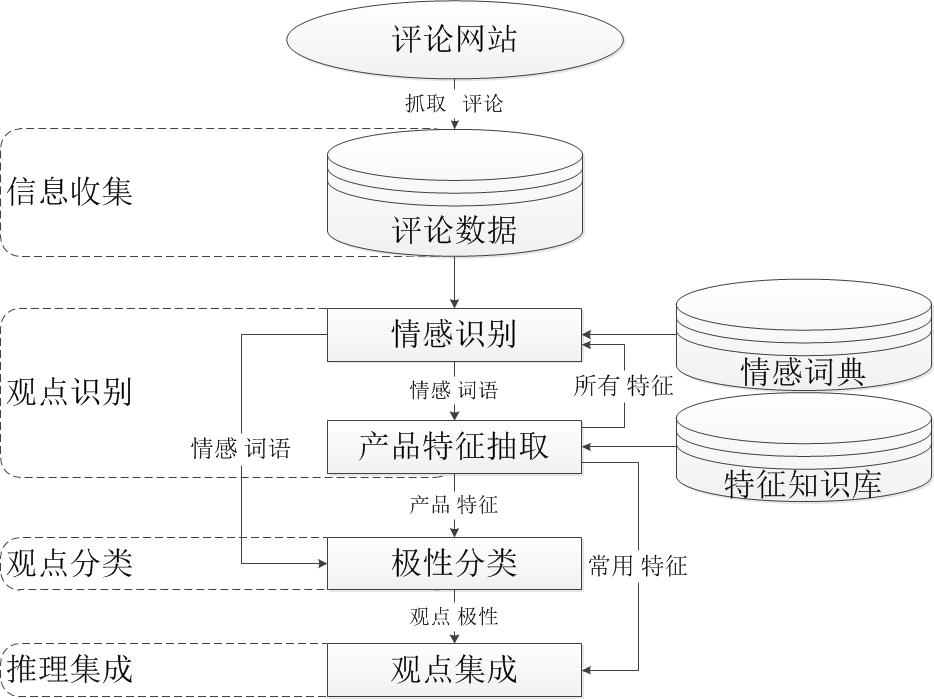
\includegraphics[height=220pt]{1-2.jpg}
\caption{产品评论的观点集成框架}
\label{fig1-2}
\end{figure}

对于文档集$ D $中的针对某话题的观点进行集成形式化表示为:
\begin{equation}
\{(f,s_f)|rep(f,D)>\rho_f,s_f=agg(S,f)\}
\end{equation}
其中$ f $表示根据某种表示度量方法$ rep(f,D) $确定的描述话题的不同方面,$ s_f $是针对$ f $根据集成函数$ agg(S,f) $计算出的针对$ f $的综合观点。

观点集成一个主要的挑战就是如何确定描述话题的多个不同方面(Aspect)。Leouski等\upcite{Leouski1996}评测了各种文本聚类方法对检索结果中信息的集成效果,发现聚类方法对于文本的交互式检索是有用的。Zeng等\upcite{Zeng2004}使用监督学习方法从文本中抽取关键短语并将其聚类用以表示话题的方面。随着话题模型的引入,越来越多的工作使用生成模型发现文档中的隐性方面话题\upcite{Su2006,Titov2008},还有一些工作使用数据挖掘中的联合规则方法对产品的相关方面进行挖掘\upcite{Liu2005,Popescu2007}。

\subsection{传播行为分析}
\label{rel3}
社交媒体中信息传播具有重要的应用价值,信息传播的主体是人,也就是社交网络的用户,研究人的传播行为是研究信息传播的重要组成部分。社交媒体中最具影响力的是微博上的信息传播,因为用户在微博的转发行为会使得信息在短时间内形成大规模的传播,因此本文主要从微博的转发行为来阐述相关工作。微博的典型代表是Twitter,Twitter转发机制,即重新发布其他人发布过的微博,以便于作者的全部粉丝看到转发的信息,使得信息迅速形成病毒式传播(Viral propagation)。很多对于转发行为的研究分析涉及影响转发行为的因素,包括tweet的文本内容与转发的关系,用户的属性如何决定其他人的转发;Twitter中信息的一般传播路径与规律等等。

相关的研究有:Boyd等\upcite{boyd2010tweet}通过实际数据研究了Twitter中转发类型和转发的原因,分析了不同用户群体,用户特性以及交流方式对于转发行为的影响,同时也从内容上分析了用户喜欢转发原因,发现微博文本中的hashtag,链接、回复、提交和转发符号都与tweet的转发存在着一定的对应关系;
Yang和Counts\upcite{yang2010understanding}研究了Twitter中用户之间提及(“@username”)关系网络,并分析了信息在提及网络上是如何传播的,发现大约有25\%的微博是被作者的朋友转发,大部分是被粉丝而非朋友转发;
Macskassy和Michelson\upcite{Macskassy2011}分析了大量Twitter用户的近一个月的数据,解释了各种信息传播的方式,尤其是转发的行为模式,发现微博的内容是被转发的决定因素;
Starbird等\upcite{starbird2012will}对危机事件发生时Twitter上的信息传播进行了深入研究,具体分析了2011年埃及的政治事件,并演示了事件的相关信息在Twitter上是生成,发展,传播过程,对于信息传播的理解有帮助作用;
Comarela等\upcite{comarela2012understanding}研究了影响用户回复或转发的因素,发现先前行为,信息发布频率,信息的时效性以及信息长度决定了用户是否回复或转发;
除了以上的工作,一些研究还从不同角度对Twitter中的转发行为机制进行了深入的研究\upcite{kupavskii2013predicting,jenders2013analyzing,ahmed2013peek,bao2013popularity}。

综上所述,影响用户转发行为的因素主要包括微博文内容、微博社交媒体特性(如是否包含链接、hashtag、提及等)、微博作者的用户特性以及社交关系等。
虽然目前Twitter转发研究从各种不同的角度进行了分析,但是还没有工作从用户的主观动机角度进行研究,本文将结合用户观点分析研究的结果对转发行为进行分析。另外,目前的转发行为分析大多都是从微博本身考虑,并未从微博接收者角度进行分析,本文将对微博、作者、接收者三个角色在转发过程中的相互关系进行探讨。

\section{研究内容与方法}

\subsection{本文研究内容}
本文研究内容主要是围绕社交媒体中用户层面的观点信息,从分析和应用两个角度对用户产生内容中的观点信息展开研究:分析角度是从不规范的社交媒体文本中挖掘观点信息,并在用户层面进行观点集成对用户的主观性进行建模;应用角度是利用用户主观模型分析社交媒体用户在线交互行为。研究框架如图\ref{fig1-3}所示。

\begin{figure}[htp]
\centering
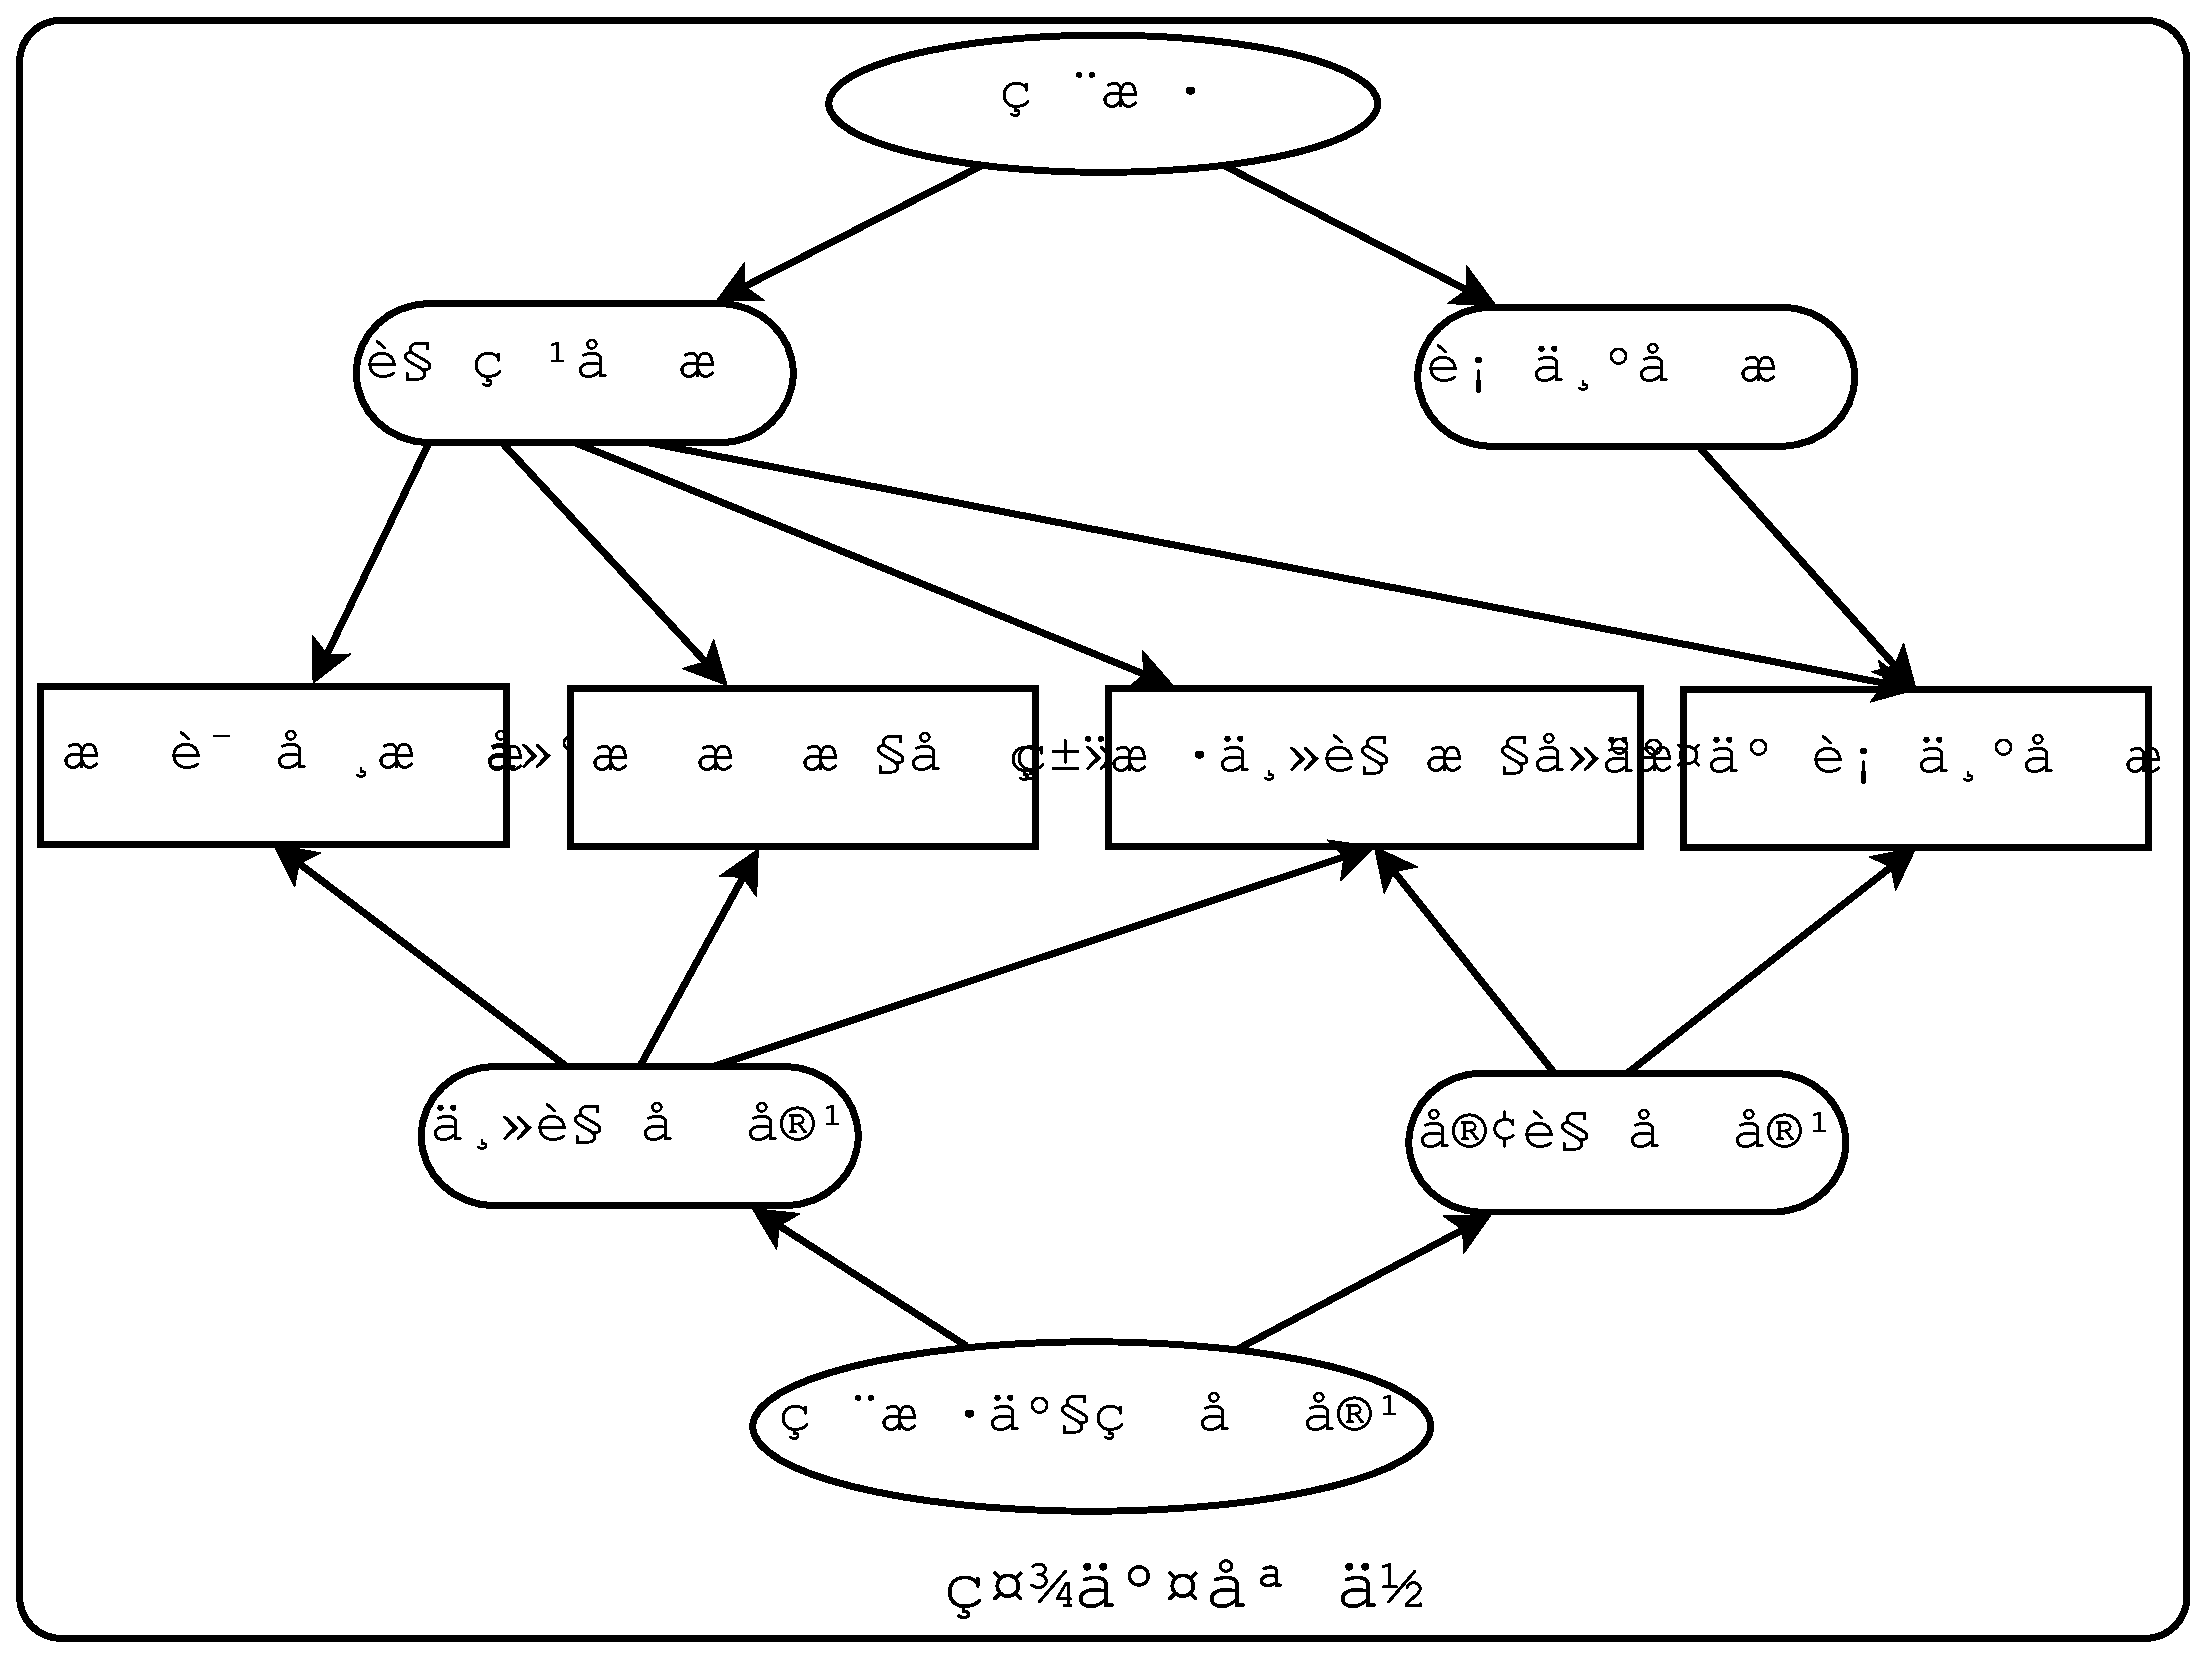
\includegraphics[height=230pt]{1-3.eps}
\caption{本文研究框架}
\label{fig1-3}
\end{figure}

本文研究内容分为四个部分:首先从社交媒体文本中得到观点信息属于观点挖掘研究内容,观点挖掘方法分为基于情感词典和基于机器学习的方法,因此需要进行\textbf{情感词典的构建}研究以及判断观点极性的\textbf{情感极性分类研究};其次从社交媒体文本片段中挖掘到的观点需要进行整合集成,变成具有代表性的观点信息,属于观点集成的研究内容,本文将从用户维度对用户的所有观点进行集成,用于\textbf{用户主观性建模};最后利用用户的主观模型,从行为主观动机角度对用户的在线交互行为进行分析,属于\textbf{交互行为分析}研究内容。
具体四个研究内容的阐述如下:

\begin{itemize}
\item \textbf{情感词典的构建}:首先对英文情感词典中的情感知识进行跨语言情感知识转化,自动构建一个通用的中文情感词典;针对通用情感词典领域适应性弱的问题,通过基于语料资源情感词典扩展研究,使用语料中的语言规则以及上下文统计特征,对情感词典在领域内进行扩展以增强情感词典的领域适应性。
\item \textbf{情感极性分类}:根据社交媒体情感表达方式的领域依赖性,对情感分类特征空间进行划分,将领域独立特征与领域依赖特征分开,首先使用两部分特征分别训练分类器,通用分类器使用现成资源训练,领域分类器使用远程监督方式训练,然后两个分类器在自举式机器学习框架下组合形成性能更好的情感分类器。
\item \textbf{用户主观性建模}:提出主观模型定义,将用户产生内容中关注的话题与针对这些话题表达的观点组合在一起对用户主观性建模。模型中对用户在每个话题上发表的所有观点进行集成,对集成的观点提出一种在情感表示空间上分布的方法来表示。基于社交媒体中用户间的网络结构,设计新的主观模型的构建方法。
\item \textbf{交互行为分析}:在构建好的用户主观模型基础上,对用户的转发行为进行分析。从主观动机角度,分析用户主观性在三种常见转发情形(即微博内容的吸引力,转发行为的社交需求以及转发行为的从众需求)中的作用,并以微博、作者和粉丝间的主观相似性进行度量。
\end{itemize}

总的来说,针对~\ref{point}的第一个科学问题,本文通过构建情感词典识别社交媒体中带有观点的文本信息,并使用无监督的情感分类方法对观点的极性进行分类,得到用户产生内容中所有观点信息;
针对~\ref{point}的第二个问题,本文通过将用户关注话题与发表的观点相结合来表示用户的主观性,并采用与话题相关的观点集成方法对用户的主观性进行建模;
针对~\ref{point}的第三个问题,本文通过计算主观模型之间的相似性度量用户信息交互行为的主观动机,进行信息转发行为分析。

\subsection{本文研究方法}
社交媒体中的观点分析涉及到机器学习、自然语言处理与自然语言理解等多方面的方法和技术,这些方法和技术的综合使用是由社交媒体文本特有的性质以及观点分析应用的特殊需求所决定的。
从社交媒体文本特性来看,进行观点分析需要面临以下挑战:
\begin{itemize}
\item 社交媒体中的文本篇幅短而且噪声多的特点,使得利用标准的机器学习方法进行分析面临数据稀疏问题,也造成自然语言处理技术的困难;
\item 庞大的数据容量以及动态的语言特性造成通用的标注数据的缺乏,无法满足机器学习训练要求;
\item 社交媒体是一个开放平台,文本涉各种领域,因此各种方法和技术都要满足多领域语境的需求;
\item 社交媒体中的数据以数据流的形式不断高速增长,需要能够快速适应新数据并能实时处理的技术和方法。
\end{itemize}

本文观点分析研究需要从大量社交媒体用户产生的内容中确定观点信息,在用户层面整合集成,然后用于分析用户的转发行为。研究中面对以上问题和挑战,需要达到如下几个目标:
\begin{itemize}
\item 使用文本规范化和消除噪音等自然语言处理技术对数据进行预处理,数据的稀疏性需要得到缓解,然后才能进入后面的分析流程;
\item 观点极性分类方法应该具有一定领域独立能力,当领域变化时能够快速适应并且性能不下降;
\item 采用的所有技术和方法能够以有限的计算能力分析和处理不断增长的数据;
\item 针对训练数据缺乏问题,尽量使用无监督或者弱监督的方法和技术,并且尽量使用已有的资源,减少人工标注。
\end{itemize}  

针对以上挑战和目标,本文确定的研究方法为:

首先在数据和资源选择上,本文首要选择已有的知识资源和标注数据。如果没有对应的知识资源,可以通过资源转化变成需要的知识资源,比如情感词典构建时,本文通过不同语言间情感知识的对应关系,将英文情感词典转化为中文情感词典。如果没有直接标注数据,本文选择采用弱标注的方法得到训练数据,所谓弱标注方法指的是,数据的类别标签是通过启发式从数据中直接确定不需要人工标注,比如在训练情感极性分类器时,本文使用含有明确情感极性的成语的微博作为训练数据,是基于微博短小,观点表达会集中在一些极性相同的词语上这一启发式,获得训练数据。在理想的情况下,用弱标记方法有两方面优势:首先,可以以很小的代价采集并标注训练数据,因此可以轻松地将相应的应用扩展到其他领域或语言;其次,弱标注方法获得标注语料的规模可以很容易达到常规手工标注方法无法获得的数量级。

在学习训练方法的选择上,本文优先选择无监督或半监督的机器学习方法。无监督或半监督学习方法可以减少或无需大量的标注训练数据,而且可以通过迁移方法将学习到的知识进行跨领域或跨语言转化。比如本文在对微博进行极性分类时,使用自举式机器学习方法将两个弱分类器结合通过迭代训练提高了分类性能;在构建主观模型时,本文使用LDA话题模型识别用户关注的话题,并使用基于规则的情感分析方法获得用户的观点信息。这些无监督和半监督方法的选择,使得本文研究过程可以减少数据选择和标注带来的人力和计算开销,提高了研究问题的抽象层级,并增强了研究方法的领域适应性和鲁棒性。

\section{本文主要贡献}
本文以用户为单位,对用户在社交媒体上产生内容中的观点信息进行识别、分析和集成,并使用用户的观点信息分析社交媒体用户在线交互行为,具体来说本文的主要贡献为:
\begin{itemize}
\item 设计了中文情感词典的自动构建和扩展方法,该方法能够从英文情感词典通过情感知识转化自动构建中文情感词典,并且能够使用领域语料进行领域内扩充,成为准确性和适应性更高的领域情感词典。通过与现有中文情感词典对比,本文的情感词典完全是自动构建,覆盖度更高,具有更好扩展性和领域适应性。
\item 基于词语在表达情感时作用的不同,提出了一种新的无监督情感分类方法,该方法将情感分类的特征空间进行划分,在两个不同的特征空间分别训练情感分类器,然后以自举式学习框架组成更好的情感分类器。方法无需人工标注的训练数据,分别使用成语词典资源和远程监督方法训练分类器,性能超过了需要大量标注数据训练的有监督分类器。
\item 提出了从用户维度进行观点集成方法,该方法将用户感兴趣话题以及在话题上的观点结合对用户主观性建模,主观模型能够在细粒度的情感表示空间中使用分布方式表示观点,用户观点表示更准确,综合反映了用户在话题每个方面所表达的观点,将该模型应用到观点预测任务时,能显著提高观点预测的准确性。
\item 从主观动机角度对用户在Twitter上的转发行为进行了分析,利用用户的主观模型设计了一种新的主观相似性计算方法,对用户转发行为的三种主观动机使用主观相似性进行度量,在真实Twitter数据中的实验中验证了三种主观相似性与转发行为之间的相关性,并且作为有效特征预测转发行为的准确性超过了目前一些主要方法,通过结合其他影响因素,可以使预测性能得到显著提升。
\end{itemize}

\section{本文结构}
本文的研究工作主要围绕社交媒体中用户的观点信息分析与应用任务展开,可以将主要工作分为以下几个主要部分:在观点分析方面,本文首先探讨了如何利用英文词典资源进行中文情感词典的自动构建,情感词典是观点信息识别和情感分类的基础;然后进一步探讨了如何结合社交媒体的文本特点对文本中表达的观点进行极性分类;最后对社交媒体中的观点信息以用户为维度进行整合集成,形成用户产生内容中表达的所有观点信息的主观模型。对分析得到的用户主观模型的应用方面,本文从用户作为信息传播的主体角度,对用户转发行为的主观动机使用主观相似性进行度量和分析。上述工作共分为七个章节,论文主体结构以及章节之间的关系如图~\ref{fig1-4}所示。,每个章节内容具体安排如下:

\begin{figure}[htp]
\centering
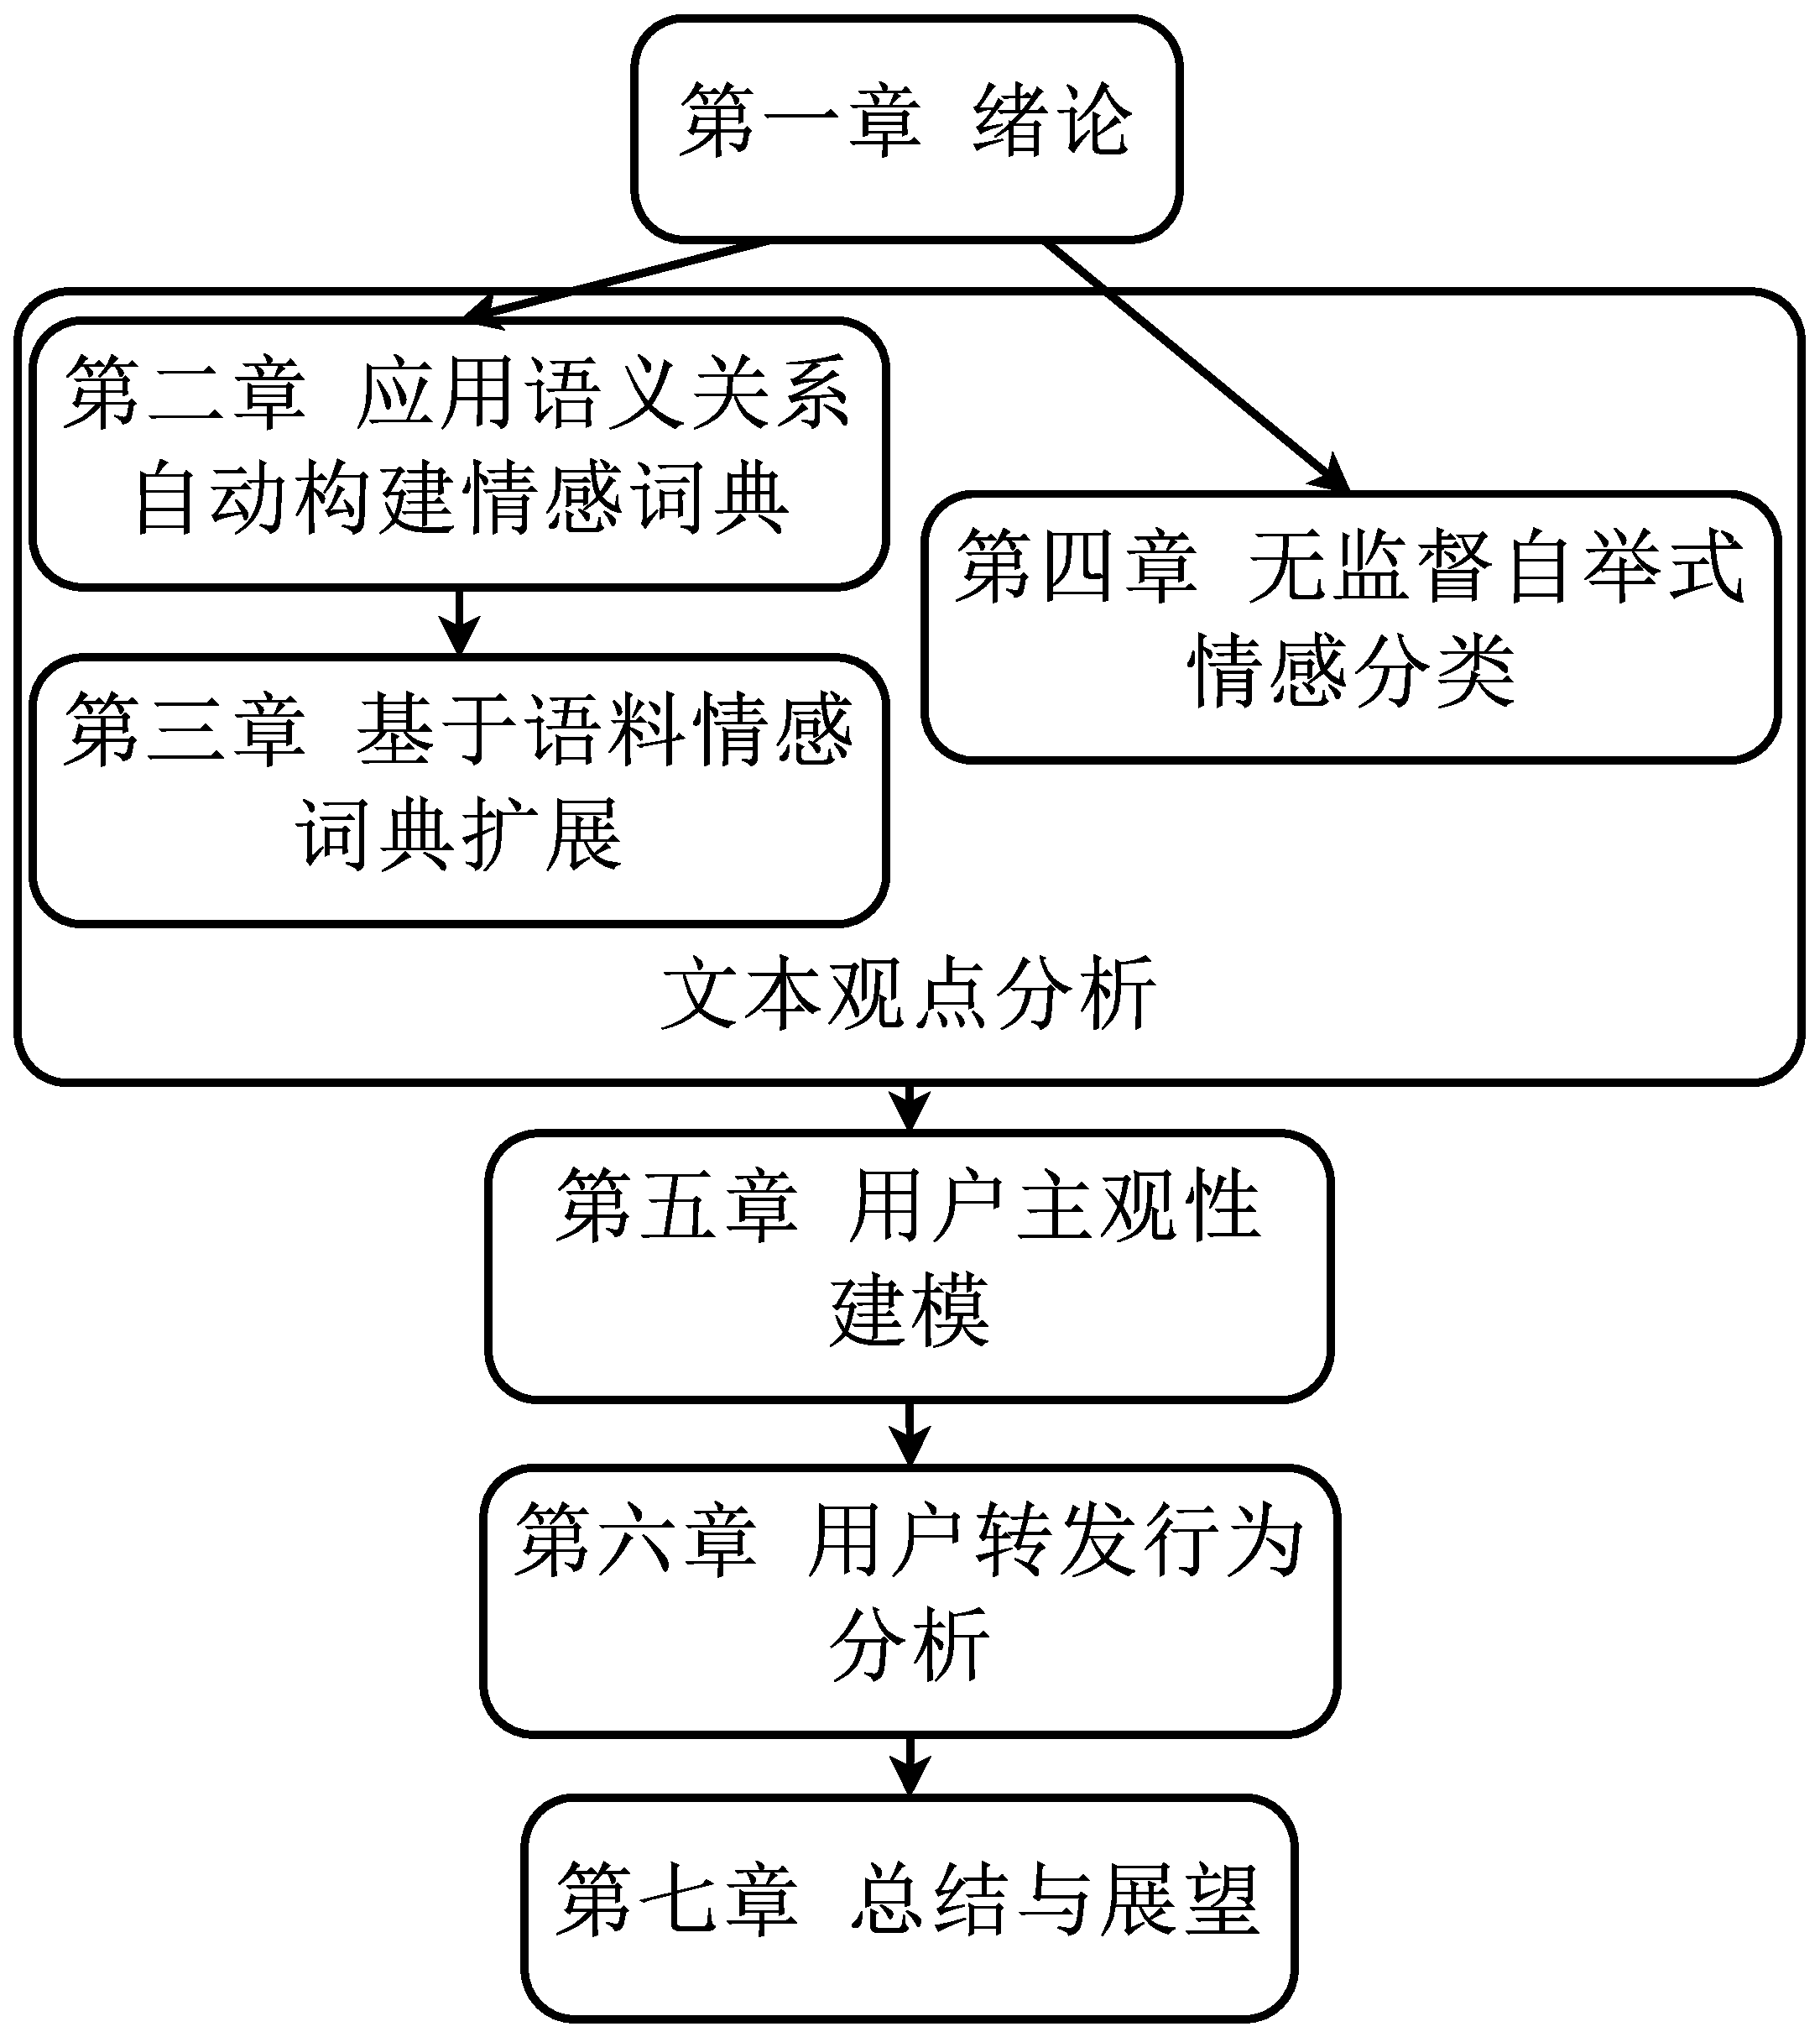
\includegraphics[height=240pt]{1-4.eps}
\caption{论文整体结构图}
\label{fig1-4}
\end{figure}

第一章是绪论,首先介绍了本文研究的背景,介绍了社交媒体和观点分析一些基础知识,接着提出研究动机,阐明了本文所涉及的科学问题、研究内容,并给出了研究方法,然后分析了研究问题,确立了依托自然语言处理技术与机器学习方法解决这些问题的基本思路,最后介绍了本文的主要工作和文章的结构。

第二章是应用语义关系自动构建中文情感词典,首先介绍了目前情感词典研究的现状,针对中文情感词典资源缺乏问题,提出了以HowNet语义知识库为基础,根据中英文词典语义之间的对应关系将英文情感词典的情感知识转化到中文情感词典中,设计了转化方法以及情感极性值的计算方法,实验中与主要中文情感词典进行了对比。

第三章是基于语料资源的中文情感词典扩展,是对第一章中构建的情感词典在领域语料中的适应性扩展的方法研究,首先介绍了基于语料资源的情感词典构建方法,确定了基于语言规则以及上下文统计特征的扩展方法,提出了综合使用两种方法的混合扩展方法,并分别进行了实验验证。

第四章是无监督的自举式情感分类,首先介绍了目前情感分类研究现状,针对领域依赖问题,根据词语在表达情感的不同作用提出了特征空间划分方法,并对研究问题进行了形式化,设计了自举式情感分类框架,选用三种常用分类器进行了实验对比分析。

第五章用户主观性建模,首先定义了社交媒体中用户的观点集成问题,然后提出了主观模型的定义,将用户产生内容中的话题和观点结合进行用户观点集成,并设计了主观模型构建方法,实验中将主观模型应用到观点预测任务,对模型进行了定性定量分析。

第六章用户的转发行为分析,研究的问题是对于给定一条微博,分析微博作者的粉丝中谁会转发该消息,针对该问题,使用主观模型从用户的主观动机角度进行分析,设计了主观相似性计算方法,并针对转发行为的三种主观动机进行度量,最后在实验中定性和定量验证了提出方法的有效性。

最后一章是总结部分,阐明了本文工作的主要贡献,并且指出了工作的一些不足,并对未来社交媒体中观点信息分析与应用的一些问题和方法进行了尝试性地思考。


\newpage 
\mbox{} 
\newpage